% rubber: set program xelatex
\documentclass[a4paper,12pt]{article}

\usepackage{xltxtra}
\usepackage{amsmath,amsthm,amssymb}

\usepackage[autostyle=true]{csquotes}
\usepackage{polyglossia}
\setmainlanguage{english}
%\setmainlanguage[variant=mono]{greek}
%\setotherlanguage{english}

% Fonts
\setmainfont{CMU Serif}
\setsansfont{CMU Sans Serif}
\setmonofont{CMU Typewriter Text}


\usepackage[xetex, colorlinks=true, citecolor=blue, linkcolor=blue]{hyperref}

% Diagrams
\usepackage{tikz}
\usetikzlibrary{shapes,arrows}

% Define block styles
\tikzstyle{decision} = [diamond, draw, fill=blue!20, 
    text width=4.5em, text badly centered, node distance=3cm, inner sep=0pt]
\tikzstyle{block} = [rectangle, draw, fill=blue!20, 
    text width=15em, text centered, rounded corners, minimum height=4em]
\tikzstyle{line} = [draw, -latex']
\tikzstyle{cloud} = [draw, ellipse,fill=red!20, node distance=3cm,
    minimum height=2em]

\usepackage{mathtools}

% Source code listings
\usepackage{listings}
\usepackage{color}
\usepackage{matlab-prettifier}
\lstdefinestyle{My-Matlab}
{
  style               = MatlabBaseStyle@mlpr,
  basicstyle          = \color{black}\ttfamily\small,
  mllastelementstyle  = \color{black}                    ,
  mlkeywordstyle      = \color[RGB]{000,000,255}         ,
  mlcommentstyle      = \color[RGB]{034,139,034}         ,
  mlstringstyle       = \color[RGB]{160,032,240}         ,
  mlsyscomstyle       = \color[RGB]{178,140,000}         ,
  mlsectiontitlestyle = \commentStyle@mlpr      \bfseries,
  mlsharedvarstyle    = \color[RGB]{000,163,163}         ,
  mlplaceholderstyle  = \mleditorphstyle,
}



\title{
\normalfont \normalsize 
\textsc{University of Burgundy \\ 
Visual Tracking
, MSCV 2018} \\
[10pt] 
\rule{\linewidth}{0.5pt} \\[6pt] 
\huge The Mean Shift Algorithm \\
\rule{\linewidth}{2pt}  \\[10pt]
}
\author{Ioannis Tsagkatakis}
\date{\normalsize \today}

\begin{document}

\maketitle
\noindent



\section{The Mean Shift Algorithm}
 In this report, an implement visual of visual tracking using mean-shift
algorithm is given. For the representation of the tracked object a metric based on the color histogram-based model is used. For the distance norm the Bhattacharyya distance is used. The algorithm is implemented in \texttt{Matlab}. The code this report as well as the results can be found in  github at \url{https://github.com/jtsagata/meanshift_tracking}.


\subsection{Initialization}
The tracker can be initialized with various methods. For example a background subtraction methods can be used. Hera we initialize the position manually and save it with the video as a \texttt{.mat} file. This method is choosed to speed up the algorithm development.

The matlab files that do the choosing and saving are:

\begin{tabular}[h]{l l}
	\texttt{demo\_cars\_prepare.m} & For the cars sequence. \\
	\texttt{demo\_head\_prepare.m} & For the head sequence. \\
	\texttt{demo\_toy\_prepare.m} & For the toy sequence. \\
\end{tabular}


\subsection{Mean-Shift tracking}
Mean-Shift considers considers that the feature space can be modeled as a probability density function (pdf). If dense regions (or clusters) are present in the feature space, then they correspond to the local maxima of the pdf. Thus the color histogram can be used as an estimator of the pdf.

The mean shift algorithm can be summarized as:
\begin{enumerate}
\item Fix a window around the traget point
\item Compute the mean data with-in the window
\item Shift the window to the mean
\item Repeat until converge
\end{enumerate}

\subsection{Object model}
The object is represent by a color distribution as showend in figure~\ref{fig:hist}

\begin{figure}[b]
        \centering
        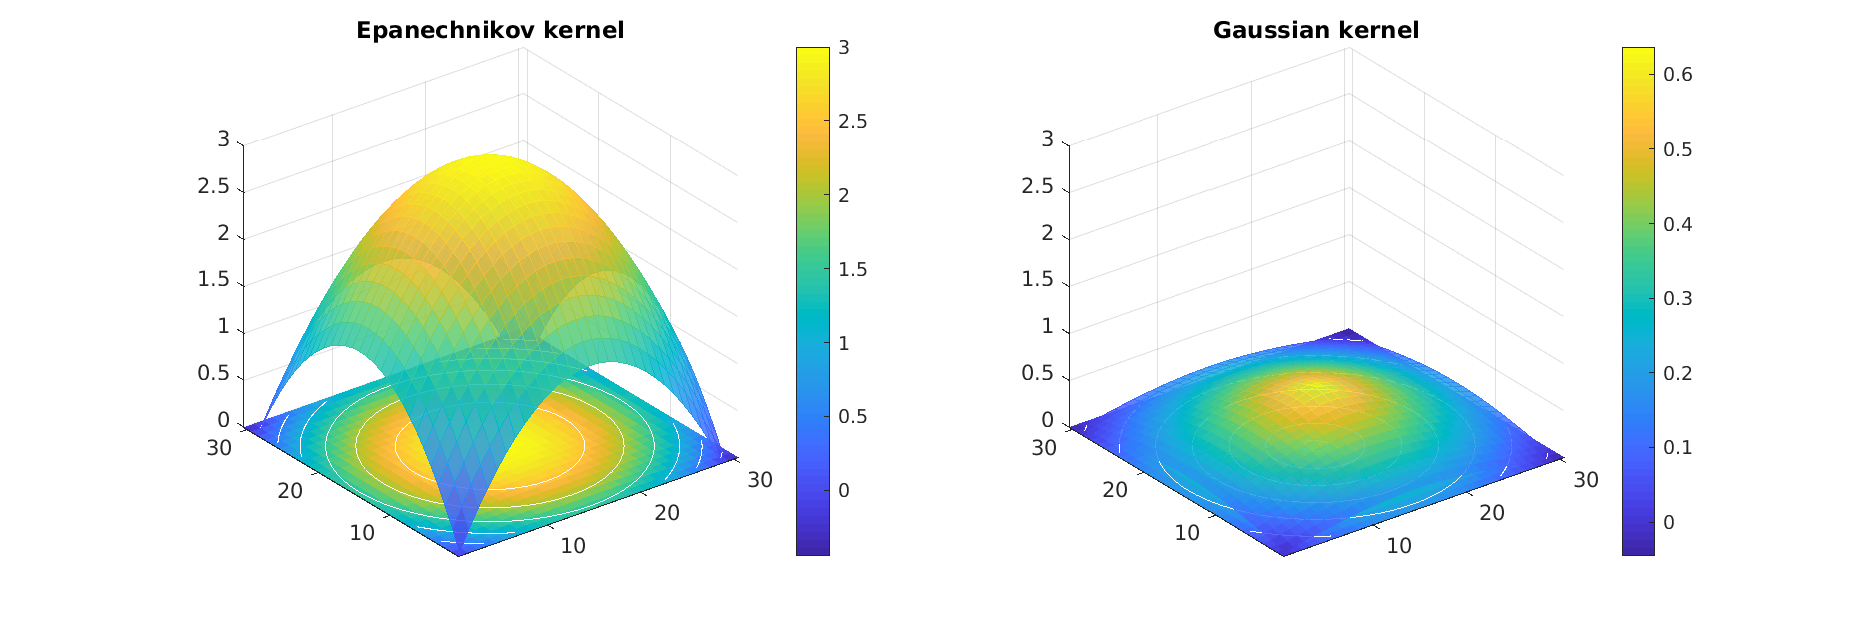
\includegraphics[width=8cm]{kernels.png}
        \caption{Common kernels}
		\label{fig:kernel}
\end{figure}




The histogram is given by the formula
$$
h(u) =  C \sum_{i=1}^{n} k\left({\left\Vert x_i \right\Vert}^2\right) \delta\left(b(x_i) - u \right)
$$
where $\left\Vert x_i \right\Vert^2$ is the normalized distace from pixel $x_i$ to the region center and $\delta(\cdot)$ is the function
$$
\delta(\alpha) = \begin{cases}
1 & when\,  \alpha=0 \\
0 & otherwise \\
\end{cases}
$$
and $C$ a normalizer. In order to take account the spatial nature of the pixels around the center location a kernel is used. A common used is the  Epanechnikov kernel given by the equation
$$
K_E(x) = \begin{cases}
\frac{1}{2}C_d^{-1}(d+2)(1 - x) & when\,  x<1 \\
0 & otherwise \\
\end{cases}
$$
where $C_d$ is the volume of the unit d-dimensional sphere. In our case, $d = 2$.

A graphical representation of an Epanechnikov and a gaussian kernel is given in figure~\ref{fig:kernel}.

\begin{figure}[h]
        \centering
        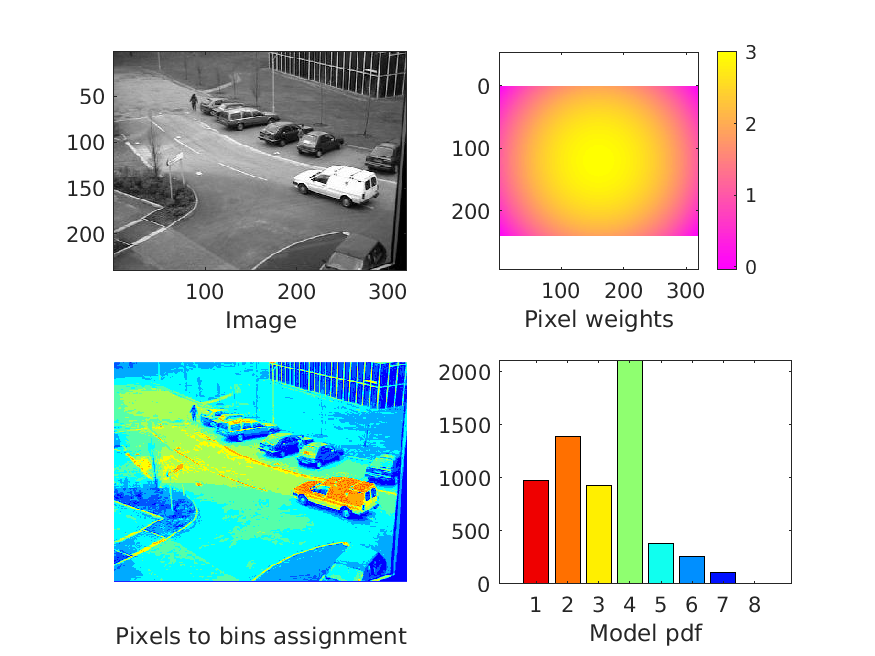
\includegraphics{historgram.png}
        \caption{Color historgram representation}
		\label{fig:hist}
\end{figure}

\subsection{Color historgram distance metric}
To estimate the similarity between a canditate location and the previous location the  Bhattacharyya metric is used, given by the formula
$$
\rho[p,q] = \sum_{u=1}^m\sqrt{q(u)q(u)}
$$
Figure~\ref{fig:hist} show the bin assignment of a frame, the kernel and the final color distribution model from a single channel image.

\subsubsection{Color distribution demos}
A video demonstration with a sliding window over an image and the color distribution is provided. 

\begin{tabular}[h]{l l}
	\texttt{demo\_algo\_meanshift\_car.m} & For the cars sequence. \\
	\texttt{demo\_algo\_meanshift\_toy.m} & For the toy sequence. \\
\end{tabular}

\noindent The resulting videos \texttt{demo\_algo\_meanshift\_car.avi} and \texttt{demo\_algo\_meanshift\_toy.avi} is on the github repository. A frame is given in figure~\ref{fig:demo1}.

\begin{figure}[h]
        \centering
        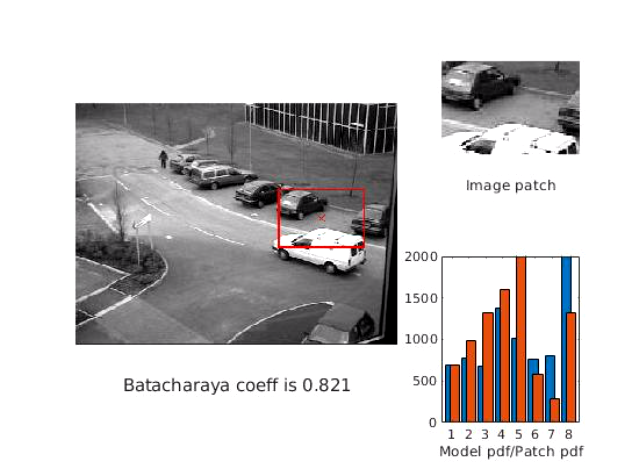
\includegraphics[width=8cm]{../Videos/demo_algo_meanshift_car.png}
        \caption{Mean shift historgram demo}
		\label{fig:demo1}
\end{figure}

\subsubsection{Matlab codes}

The file \texttt{kernelMatrix.m} calculates a kernel of size $n\times{}m$.

\lstinputlisting[style=My-Matlab]{../Code/kernelMatrix.m}

The file \texttt{bhattacharyya\_coeff.m} calculates the Bhattacharyya metric. The file \texttt{histDistMat.m} distributes pixels to histogram bins. The file \texttt{color\_distribution.m} calculates the color distribution of a monochrome or RGB image. Note than an \texttt{eps} is added to every value, in order  to avoid zero elements.
\lstinputlisting[style=My-Matlab]{../Code/color_distribution.m}


\subsection{The tracking algorithm}
The code that implements the mean shift tracking is given bellow. In order the algorithm not enter into infinite or large loops $loop\_count$ and $rho\_loop\_count$ variables limits the number of iterations.

\lstinputlisting[style=My-Matlab]{../Code/meanshift_algorithm.m}

\noindent The code that calculates the mean shift vector is given bellow. Note that the code works for for both grayscale and RGB images. The code is hightly optimized and vectorized.
\lstinputlisting[style=My-Matlab]{../Code/meanshift_vector.m}


\noindent The code to calculate the meanshift weights is also presented here. The values of the weight matrix there always be bigger than zero by starting with a small \texttt{eps} value.
\lstinputlisting[style=My-Matlab]{../Code/meanshift_weights.m}


\subsection{Support code}
Please look at the github repository\footnote{\url{https://github.com/jtsagata/ meanshift_tracking}} for the rest of the support code. A lot of operations have been put in a custom matlab object called \textt{xROI} that represent a region of interest of an image. A region of interest knows his top left, center and bottom right coordinates and the center location. It can scale and get subimages and color distributions among other operations. Look at the files \texttt{xRoi.m} for the implementation and at \texttt{xRoi\_test.m} for some basic usage and testing.


\section{Mean Shift applications and demos}
In the repository theres is the code for the following demos 

\begin{tabular}[h]{l l}
	\texttt{demo\_cars.m} & Basic car demo\\
	\texttt{demo\_cars\_adaptive.m} & Recalculates the histogram at each run (failed).\\
	\texttt{demo\_cars\_varsize.m} & Adapt frame size (good results)\\  
	\texttt{demo\_head.m} & Heads demo \\
	\texttt{demo\_head\_varsize.m} & Adaptive heads demo\\
	\texttt{demo\_toy.m} & Toy sequence demo (bad results)\\
	\texttt{demo\_toy\_varsize.m} & Adaptive toy sequence (bad results) \\
\end{tabular}

\noindent each demo loads the video and the tracking roi from a \texttt{.mat} file, runs the tracking algorithm and save the video result. Also its saves a picture with selective frames from the video and a text file containing timing information. The resulting files are in the github repository.

\begin{figure}[h]
        \centering
        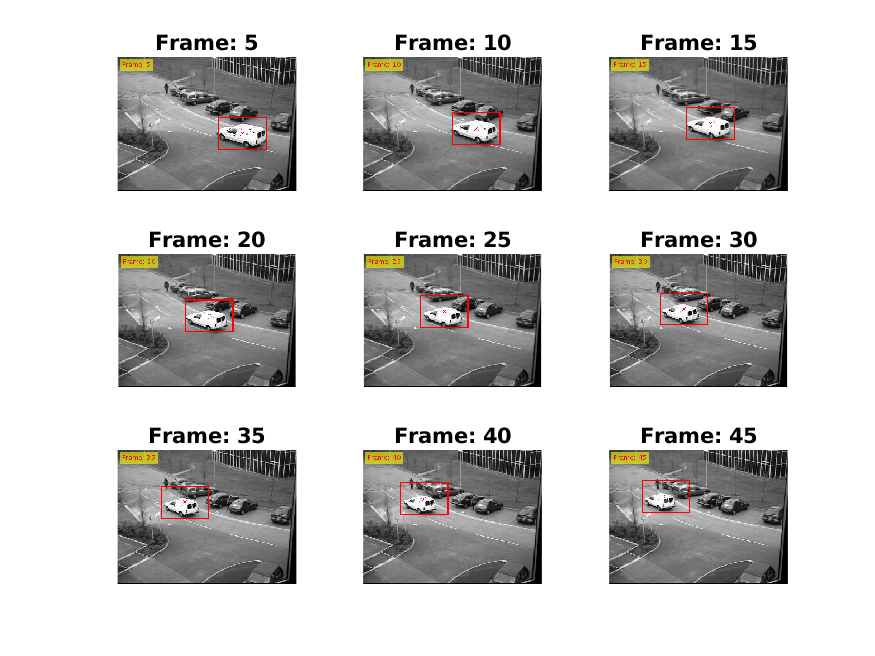
\includegraphics[width=8cm]{../Videos/demo_cars.png}
        \caption{Car sequence simple demo}
		\label{fig:demo2}
\end{figure}
\newpage
Some frames for the car sequence is given in figure~\ref{fig:demo2} and in figure~\ref{fig:demo3} when we adapt the frame window. The tracking result is quite good and computationally applicable.

\noindent In my laptop the execution times are

\begin{tabular}[h]{l l}
	\texttt{demo\_cars.m} & 42.9381 secs\\
	\texttt{demo\_cars\_varsize.m} & 31.1478 (smaller)\\  
\end{tabular}


 

\begin{figure}[ht]
        \centering
        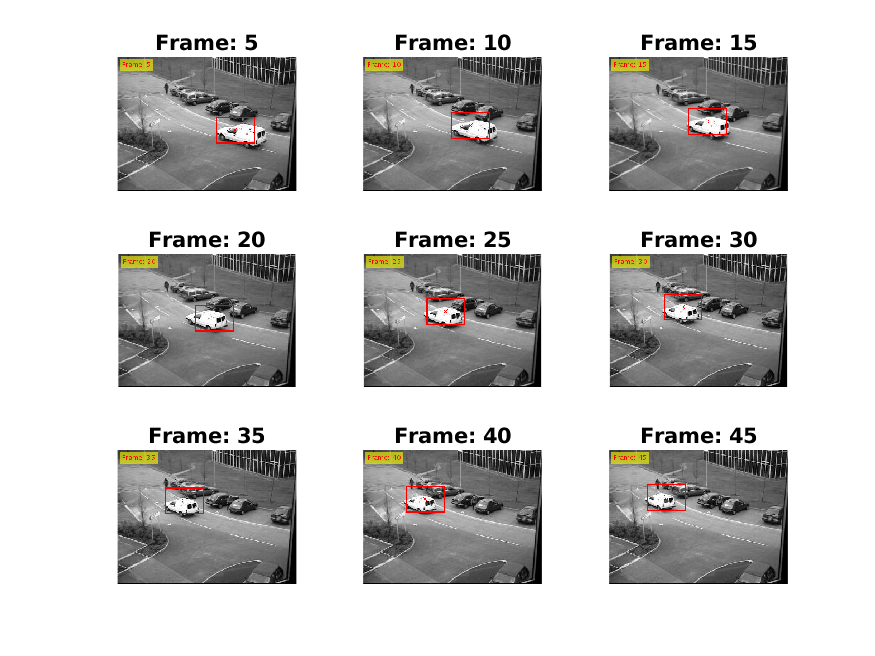
\includegraphics[width=8cm]{../Videos/demo_cars_varsize.png}
        \caption{Car sequence variable roi size demo}
		\label{fig:demo3}
\end{figure}




%\begin{figure}[h]
%        \centering
%        \\begin{figure}[h]{../Videos/demo_algo_meanshift_car.png}
%        \caption{Distance demo}
%\end{figure}


% USE NOCITE TO ADD SOURCES TO THE BIBLIOGRAPHY WITHOUT SPECIFICALLY CITING THEM IN THE DOCUMENT

%\nocite{ref_num}


%%%%%%%%%%%%%%%%%%%%%%%%%%%%%%%%%%%%%%%%%%%%%%%%%%%%%%

			% BIBLIOGRAPHY: %

% Make sure your class *.bib file is uploaded to this project by clicking the project button > add files. Change 'sample' below to the name of your file without the .bib extension.
%%%%%%%%%%%%%%%%%%%%%%%%%%%%%%%%%%%%%%%%%%%%%%%%%%

%\bibliographystyle{plainnat}
%\bibliography{sample}

% UNCOMMENT THE TWO LINES ABOVE TO ENABLE BIBLIOGRAPHY

%%%%%%%%%%%%%%%%%%%%%%%%%%%%%%%%%%%%%%%%%%%%%%%%%%


\end{document} % NOTHING AFTER THIS LINE IS PART OF THE DOCUMENT
